%% General definitions
%\documentclass{IEEEtran}
\documentclass{article} %% Determines the general format.
\usepackage{a4wide} %% paper size: A4.
\usepackage[utf8]{inputenc} %% This file is written in UTF-8.
%% Some editors on Windows cannot save files in UTF-8.
%% If there is a problem with special characters not showing up
%% correctly, try switching "utf8" to "latin1" (ISO 8859-1).
\usepackage[T1]{fontenc} %% Format of hte resulting PDF file.
\usepackage{fancyhdr} %% Package to create a header on each page.
\usepackage{lastpage} %% Used for "Page X of Y" in the header.
                      %% For this to work, you have to call pdflatex twice.
\usepackage{enumerate} %% Used to change the style of enumerations (see below).
\usepackage{amssymb} %% Definitions for math symbols.
\usepackage{amsmath} %% Definitions for math symbols.
\usepackage{graphicx}

\usepackage{float}

%% Left side of header
\lhead{\course\\\semester\\Report 1}
%% Right side of header
\rhead{\authorname\\Page \thepage\ of \pageref{LastPage}}
%% Height of header
\usepackage[headheight=36pt]{geometry}
%% Page style that uses the header
\pagestyle{fancy}

\newcommand{\authorname}{Elias Arnold\\Alexander Luyten}
\newcommand{\semester}{Spring semester 2019}
\newcommand{\course}{43075-01 Probabilistic Shape Modelling}
\author{Elias Arnold and Alexander Luyten}

\title{Project: Reconstruction of Partial Femurs}

\begin{document}
\maketitle
\section{Introduction}
The aim of this project is to reconstruct a partial femur bone with the help of a self-constructed femur model. Shape-reconstructions have a wide-ranged purpose especially in the medical field for modelling implants.\par
In our case, the model is built using real-world data of 50 femur scans from patients and is called a Statistical Shape Model (SSM). It consists of a reference shape and a distribution over deformations fields. To obtain a final femur reconstruction we first perform registration of our model to every partial femur bone, this gives us full correspondence between the two shapes. We then compute the most likely explanation of our final model to the missing shape.

\section{Methods}
\subsection{Rigid Alignment}
First, we had to align all the given femur bones to a reference shape, which means that we had to find a translation and a rotation for each bone so that all the squared differences of the points in the two meshes are minimal. This can be expressed as a minimization problem, which can be efficiently solved using singular value decomposition.\par
We can now perform registration between our model and the target shapes to establish correspondence, mentioned in subsection \ref{establishing_correspondence}.

\begin{figure}[H]
	\begin{minipage}[t]{0.45\linewidth}
		\centering
		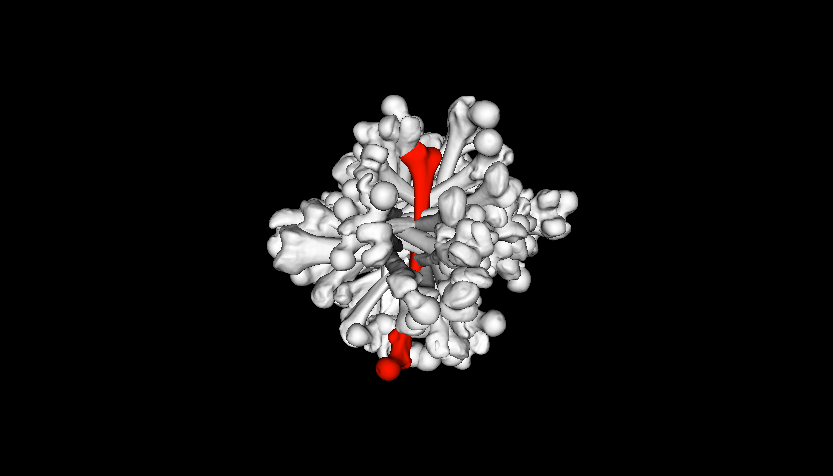
\includegraphics[width=.9\textwidth]{img/unaligned_bones.png}
		\caption{All the 50 target shapes (white) and the reference bone (red). We cannot fit a model to the target shapes, because their orientation is arbitrary.}
		\label{fig:unaligned_bones}
	\end{minipage}
	\hfill
	\begin{minipage}[t]{0.45\linewidth}
		\centering
		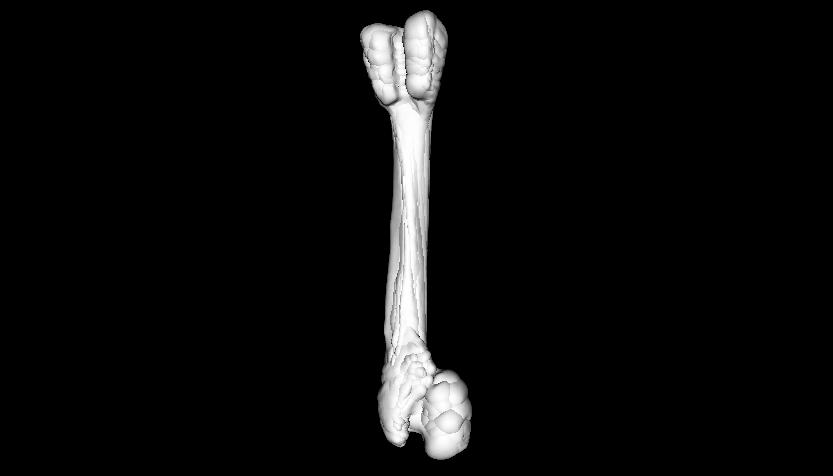
\includegraphics[width=.9\textwidth]{img/aligned_bones.png}
		\caption{The 50 target bones again, but aligned to the reference shape. It is not visible since it gets occluded from all other bones.}
		\label{fig:aligned_bones}
	\end{minipage}
\end{figure}

\subsection{Building a Model}
In the second step, we built a first femur bone model. As mentioned before, we created a Statistical Shape Model containing a reference shape and a Gaussian Process (GP). A Gaussian Process is a normal distribution over deformation fields and is defined by a mean and covariance function. In our case, the mean function is the zero vector and the covariance function is computed from a combination of hand-crafted kernels.\par
As we want to model the shape variation of the femur bone as closely as possible, we thought about certain properties, that the femur bone model should have:
\begin{itemize}
\item The femur model should capture the ability of the femur bone to grow or shrink
\item The width of the bone model should correlate with the length of the femur bone model
\item The joints should mildly be influenced by the length of the bone, but should be uniformly stretched in every direction and not in one single direction. We assumed, that the hip joint should stay round independently of the size of the shaft.
\end{itemize}
We tried to model these properties with a combination of different kernels: A Changepoint-Kernel which handles the shaft and the joint region differently, and a Diagonal-Kernel with small variance, to capture fine-grain deformations. As we have to specify the transition $s(p)$, we had to determine the regions where each kernel should be active. We first chose a z-coordinate threshold, which resulted in a very abrupt kernel change. To alleviate this problem, we used a combination of two logistic functions:
\begin{equation}
\label{Formula}
s(p) = \Big(1 - \frac{1}{1+ke^{-k(p(z) + \textit{LJoint})}}\Big) + \frac{1}{1+ke^{-k(p(z) - \textit{UJoint})}}, \text{ where } k = 0.1 
\end{equation}
Here $\textit{LJoint}$ and $\textit{UJoin}$ are the upper and lower joint cutoff regions in equation (\ref{Formula}).

\begin{figure}[H]
	\centering
	\begin{minipage}[h]{0.45\linewidth}
		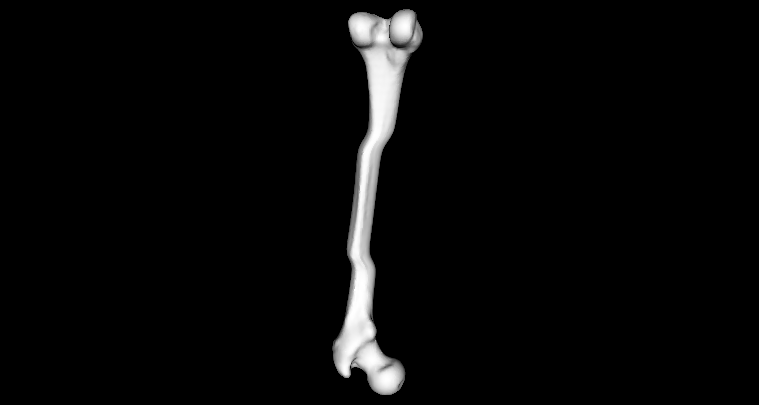
\includegraphics[width=.9\textwidth]{img/changepoint_kernel.png}
	\end{minipage}%
	\centering
	\begin{minipage}[h]{.45\textwidth}
		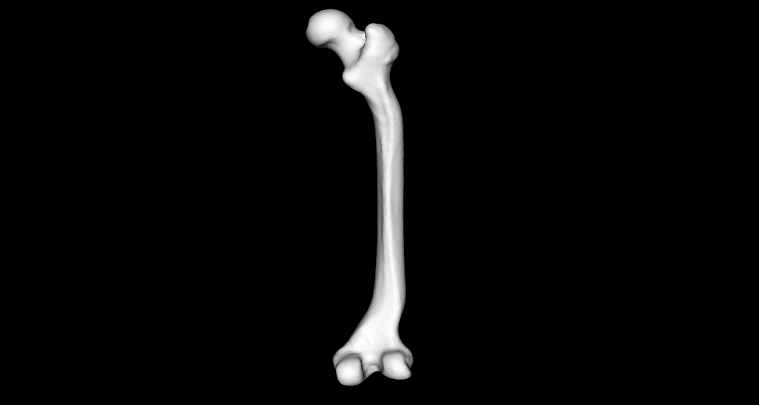
\includegraphics[width=.9\textwidth]{img/changepointkernel2.png}
	\end{minipage}
	\caption{Left-hand-side: Our first approach to use a different kernel for the joints than for the shaft of the bone. As seen, we wrongly chose a low cut-off value for the joint regions. Also the transition was not smooth enough for our purpose. Right-hand-side: The final Changepoint-Kernel with a smooth transition. In both images, the independence of the two parts is pushed to the limit to demonstrate the effect of the two separate kernels.  Therefore, both shapes are very unlikely.}
	\label{fig:changepoint_kernel}
\end{figure}

\subsection{Establishing Correspondence}
\label{establishing_correspondence}
In order to build a model that captures all real-life deformations, we have to find the deformation fields between our reference shape and all 50 target femur bones. As we don't have a direct correspondence between all points in every shape, we have to use an algorithm which establishes correspondence. We used ICP, short for Iterative Closest Point algorithm, which is a heuristic for computing the point correspondence. The algorithm works by iteratively finding the closest points between target and reference points, estimating a transformation based on these corresponding points, and transforming the reference using this transformation.\par
To be able to evaluate our registration, we compared our resulting mesh with the given target mesh using the average distance. We computed an average value of 0.82 mm for all 50 target meshes.

\subsection{Final Model}
Our final model is built with the 50 femur bones using Principal Component Analysis (PCA). After computing the deformation fields, we are able to build the final SSM. As the resulting covariance matrix of the GP can be too large to fit into memory an approximation of this covariance matrix can be computed using the Karhunen-Loève Expansion. This procedure lets us extract only the most important basis functions from the model in Low-Rank Approximation and find extrema of the probability distribution because of the closed form.\par

\subsection{Reconstruction}
For the last step - the fitting of the model to the partial femurs - we used the ICP algorithm as well. However, the deformation vectors were calculated from the partial femur to the model, in contrast to the usual way, where we computed the vectors in the opposite direction. We had to do it like this because it is not guaranteed that every point of the model has a counterpart on the contour of the target shape, seen in Figure \ref{fig:reconstruction}.\par
After fitting our model to the partial femur, we compute the posterior distribution, where the given partial shape is the data and our model is the prior distribution. Our reconstruction, in the end, is the mean of this posterior distribution, as this is the most likely explanation.
\begin{figure}[H]
	\centering
	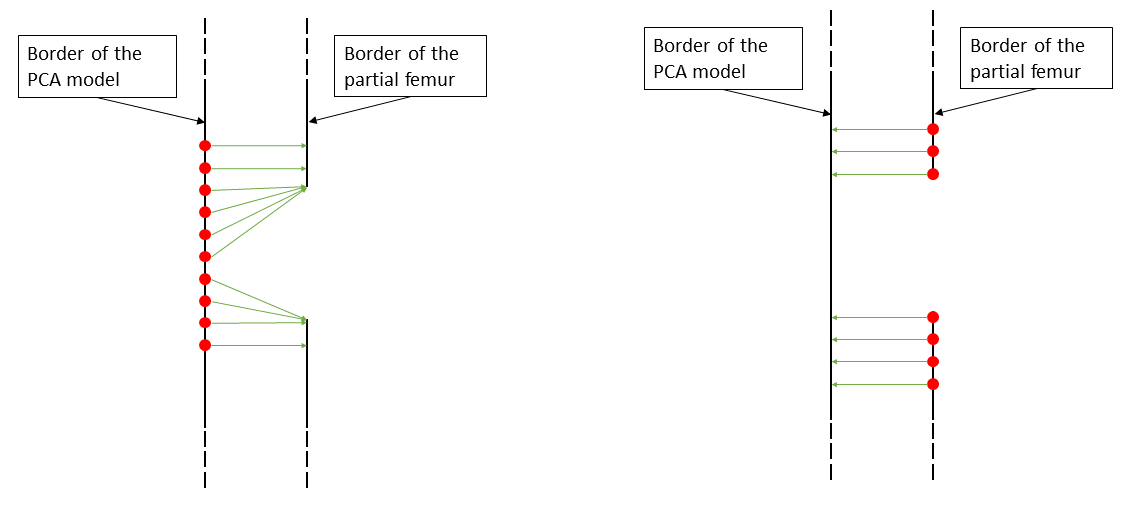
\includegraphics[width=0.8\textwidth]{img/reconstruction_ICP_cut.png}
	\caption{On the left-hand side, we see the deformation field if the vectors would originate on the model. The right-hand side shows the opposite direction of the vectors. It can be seen that the resulting deformation field is smooth, although it has gaps.}
	\label{fig:reconstruction}
\end{figure}

\section{Results}
\label{results}
We were able to reconstruct nearly all of the partial femurs correctly. However, there was one reconstruction that failed. After comparing the failed reconstruction with our target mesh, we think that our model isn't able to capture the full length of the target, as the target femur seems above average in length. To overcome this problem, we will have to adjust our initial model by reviewing the used kernels.\par
The rest of the successfully reconstructed femurs look natural and also fit very well around the given partial shapes, especially around the joints. The trade-off in this kernel was the $\sigma$ parameter, which controlled the correlation between the deformation vectors. If it was chosen too low, there was too much leeway for the model and vice versa, seen in figures \ref{fig:badModel} and \ref{fig:goodModel}.\par
We participated in the SMIR contest and ended up in the 28th rank, which was in the middle of the ranking. This result wasn't all too surprising, as one reconstruction failed. Future optimizations for an improved reconstruction error could be done, by sampling more points in the fitting and registration process. We also tried improving our Changepoint-Kernel approach, but could not figure out, which kernel was responsible for the failed reconstruction.

	\begin{minipage}[t]{0.45\linewidth}
	\begin{figure}[H]
		\centering
		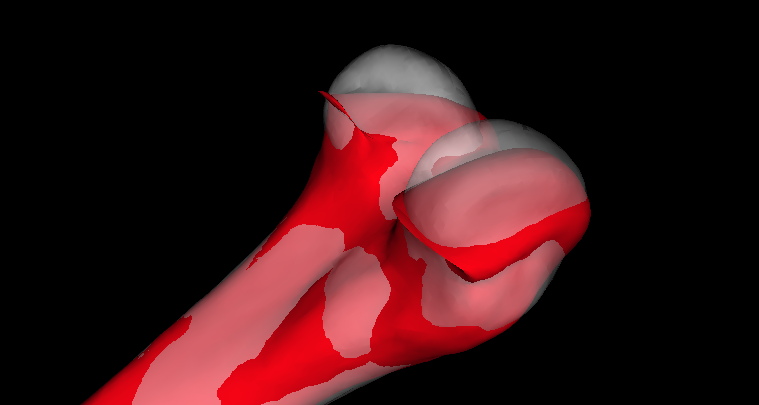
\includegraphics[width=.9\textwidth]{img/badModel.png}
		\caption{Although the registration of the small variance model (red) on a given bone (transparent) has little numerical error, it is not a valid shape of a femur bone.}
	    \label{fig:badModel}
	\end{figure}
	\end{minipage}
	\hfill
	\begin{minipage}[t]{0.45\linewidth}
	\begin{figure}[H]
		\centering
		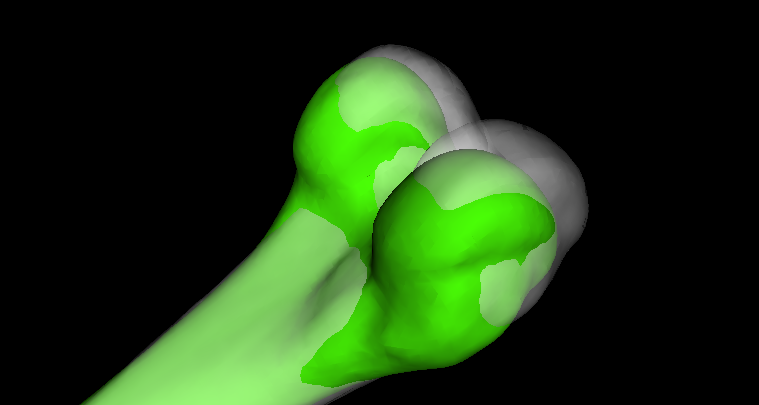
\includegraphics[width=.9\textwidth]{img/goodModel.png}
		\caption{If we perform registration between a model with larger variance (green) and given femur scan, the numerical error is larger, but it remains an anatomically valid shape.}
	\label{fig:goodModel}
	\end{figure}
	\end{minipage}

\section{Conclusion}
The goal of this project was to complete partial bone scans. For this, a model of a bone is deformed in a way, that it explains the existing part of the bone as well as possible. Then, a probability distribution on the missing parts of the bone can be calculated, which suggests how the bone most likely looked like.\par
Initially, we had given 50 pairs of femur bone shapes and landmarks. As a first step, we rigidly aligned all bones to a reference bone. After that, we created an SSM with hand-crafted kernels reflecting our ideas on how the femur shape variation should look like. Afterwards, we performed registration between the handcrafted model and the given bones, which allowed us to calculate the deformation fields. These were then used to create the final femoral bone model, which was then used for the reconstructions.\par

Throughout the project, we have learned that it is important to extensively review the results after each step. It can be very time-consuming to look for a mistake in the past as it can have happened in every step taken so far. In the final step of the project, we suddenly realized that our model for the reconstructions allowed deformations that were anatomically impossible. It took us a lot of time to realize that we should not use kernels with a combination of a low variance and a big scale because otherwise, the model has too much leeway and can represent shapes that look unnatural.\par

We think that the idea with the Changepoint-Kernel should be investigated further, since the bone joints in each case should be a round sphere, while the bone shaft can be stretched arbitrarily. We have decided not to give our kernels many liberties (large $\sigma$), which tends to produce a big numerical error during registration or fitting.\par

\begin{figure}[H]
		\centering
		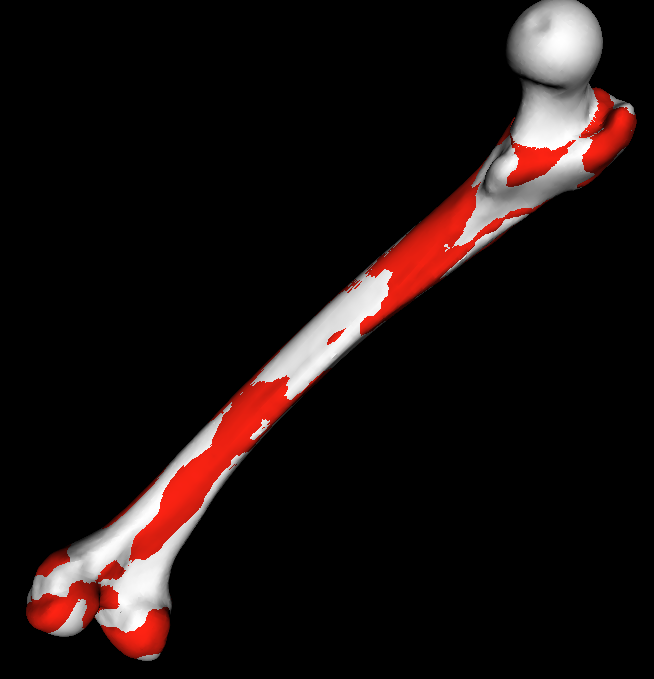
\includegraphics[width=.6\textwidth]{img/newest.png}
		\caption{Received successful femur bone reconstruction, here the red area belongs to the partial femur and the white bone is our reconstruction.}
	\end{figure}
\end{document}